\chapter{Design}
Per lo sviluppo e l'implementazione del sistema è stato scelto lo stack MERN, una variazione dell'originale stack MEAN \cite{meanWikipedia} nella quale Angular viene sostituito da React. Questa architettura permette di creare in maniera semplificata una struttura su tre livelli (\emph{front end, back end, database}) utilizzando solamente JavaScript e JSON.

\begin{figure}[H]
\centering

\includegraphics[width=0.4\textwidth]{img/logos/MERN-logo.png}
\caption{Tecnologie stack MERN}
\label{fig:mern}
\end{figure}

Per quanto riguarda invece le interazioni tra le parti del sistema è stato scelto di utilizzare un'architettura ibrida tra \emph{Client-Server} e \emph{Peer-to-Peer}. Come si può vedere in figura \ref{fig:architettura} il server sarà il punto di snodo tra i client ed il database, svolgendo inoltre la funzione di \emph{discovery server} per quanto riguarda le reti p2p. Ogni client sarà quindi in comunicazione con il server per le funzioni di autenticazione, discovery ed interazioni con il db, ma una volta entrato in un \emph{party} sarà connesso direttamente agli altri client.

\begin{figure}[H]
\centering
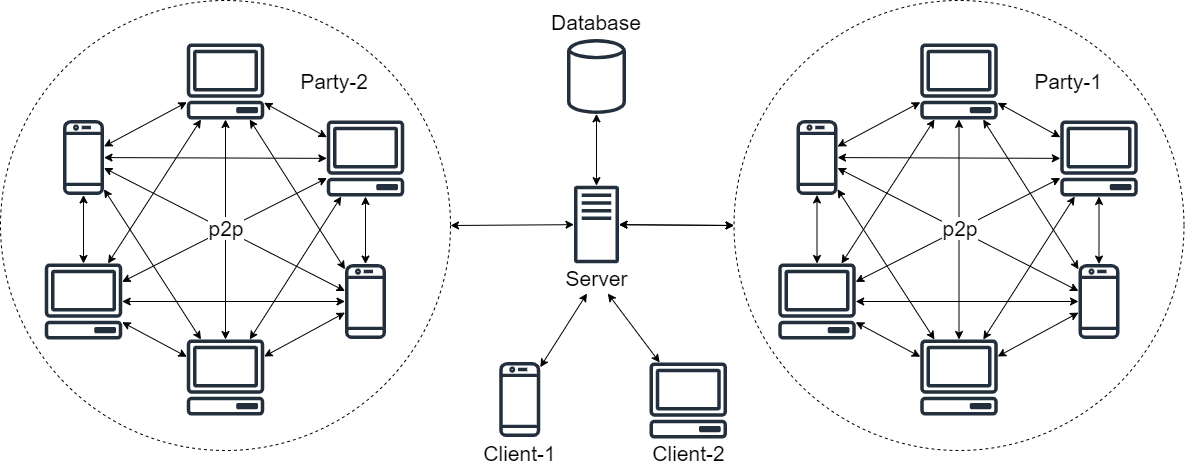
\includegraphics[width=\textwidth]{img/architettura.png}
\caption{Sintesi architettura del sistema}
\label{fig:architettura}
\end{figure}


\section{Struttura del Server} \label{serverStruct}

Il server come detto in precedenza si basa sul framework Express, in accordo con lo stack MERN, e svolge il ruolo di \emph{discovery} per i client che si connettono. Sfruttando la libreria Mongoose all'avvio viene effettuata la connessione al database, dopodiché vengono impostate le route per le richieste HTTP e gli handler per i messaggi ricevuti attraverso le web-socket.\\

Al fine di evitare una crescita incontrollata delle comunicazioni nel caso il sistema venga scalato ad un utilizzo più esteso sono state utilizzate le \emph{rooms} \cite{socketIORooms} messe a disposizione dalla libreria, ovvero dei canali di comunicazione ai quali le socket possono unirsi che permettono al server di inviare messaggi a specifici sottoinsiemi di client senza effettuare broadcast delle informazioni. La singola room corrisponde come concetto a quello di party descritto in precedenza, rappresentando quindi un gruppo di giocatori logicamente isolato dagli altri.

\subsubsection*{Socket}
Per stabilire la connessione tra client e server è stata utilizzata la libreria Socket.io. Per la gestione delle sessioni viene utilizzato un \emph{middleware} \cite{socketIOMiddlewares} che permette di generare identificatori univoci per gli utenti autenticati, dato che l'identificativo del peer viene rigenerato ogni volta, e recuperare quelli presenti in memoria per quelli che ripristinano una connessione.\\
Quando il server riceve una richiesta di connessione da parte di un client viene richiamato il primo handler, \textit{io.on('connection'...)}, che andrà ad associare alla socket tutti gli altri handler, nel codice creati con \textit{socket.on('name', (message)...)}, qui di seguito riportati solo per nome e descrivendo l'eventuale messaggio atteso.

\begin{itemize}
    \item \textbf{disconnect}: Messaggio inviato in automatico dal client al momento della disconnessione, il server modifica lo stato della sessione come non connesso, e lo rimuove dalla room.
    \item \textbf{logout}: Quando un utente effettua il logout l'identificativo associato alla sua sessione viene cancellato completamente.
    \item \textbf{login}: Inviato con un payload contenente username e password, se l'autenticazione va a buon fine viene inviato come risposta e salvato localmente il codice della sessione, diversamente verrà inviato un messaggio di errore.
    \item \textbf{signup}: Anche nel caso della registrazione i campi del payload saranno sempre username e password, la risposta sarà positiva o negativa a seconda dell'esito del salvataggio delle credenziali sul database.
    \item \textbf{room}: Questo messaggio richiede due identificativi, uno per identificare il peer ed uno per la room alla quale ci si vuole unire. Il server a seconda dello stato della room avrà comportamenti leggermente diversi, tutti finalizzati alla comunicazione degli identificativi dei peer ai client della room stessa, facendo sì che tutti possano connettersi tra di loro e formare una effettiva rete p2p.
    \item \textbf{close\_room}: Con l'identificativo della room come payload serve per comunicare al server che nessun altro client potrà più unirsi al canale.
    \item \textbf{peer\_destroyed}: Se il peer viene distrutto completamente verrà anche in questo caso rimosso dalla room e in più l'evento sarà comunicato a tutti i partecipanti alla stessa.
    \item \textbf{save}: Inviato con un payload contenente tutte le informazioni relative alla partita appena conclusa si occuperà di salvarle sul database.
    \item \textbf{send\_stats}: Inviato con uno username come payload risponde inviando tutte le informazioni e statistiche correlate allo storico del giocatore.
    
\end{itemize}


\subsubsection*{Routes}
Per quanto riguarda le richieste HTTP il server utilizza il Router fornito da Express. In una prima fase di sviluppo queste route sono state utilizzate per interagire con il server ed il database, successivamente poi nelle versioni più avanzate del sitema ne sono state mantenute solo alcune ai fini di offrire la possibilità all'utente che esegue il server di visualizzare alcune informazioni utili. Le route in aggiunta a quella di default \emph{"/"} sono divise come segue:

\begin{itemize}
    \item User:
    \begin{itemize}
        \item \textbf{GET - /users}: Ritorna le informazioni relative a tutti gli utenti registrati al server.
        \item \textbf{GET - /user/:username}: Ritorna le informazioni dell'utente identificato dallo username.
        \item \textbf{POST - /user} : Prendendo come parametri username e password crea un nuovo utente nel database.
    \end{itemize}
    \item Game:
    \begin{itemize}
        \item \textbf{GET - /games}: Ritorna le informazioni relative a tutte le partire giocate e salvate sul server.
    \end{itemize}
            
\end{itemize}


\newpage
\section{Struttura del Database}
Il database utilizzato dal sistema è stato strutturato in maniera semplice con l'obiettivo di familiarizzare con le tecnologie impiegate, raggiungendo comunque i requisiti che erano stati prefissati.\\

\begin{figure}[H]
\centering
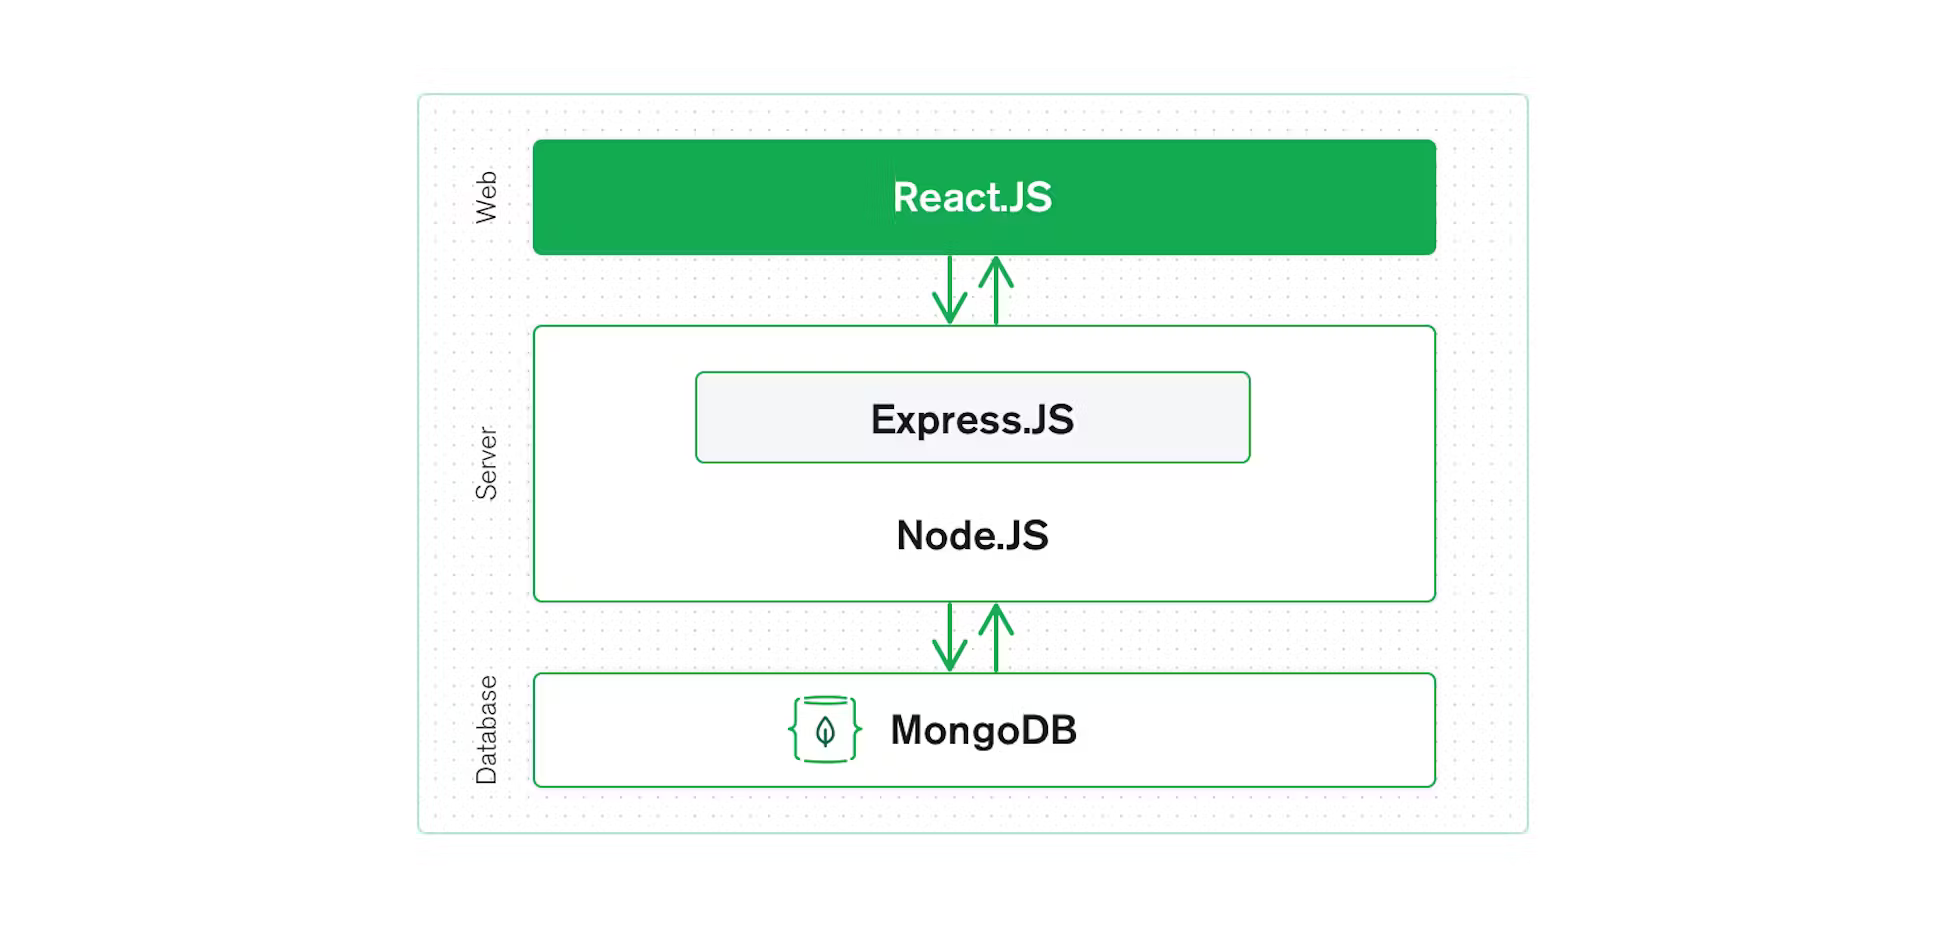
\includegraphics[width=\textwidth]{img/mern-stack.png}
\caption{Stack MERN \cite{mongodbMERN}}
\label{fig:mongodbmern}
\end{figure}


\begin{figure}[H]
\centering
\includegraphics[width=0.8\textwidth]{img/db-classes.png}
\caption{Diagramma delle classi}
\label{fig:dbClasses}
\end{figure}


Come si può vedere nella figura \ref{fig:dbClasses} le informazioni salvate si riassumono in due classi, \emph{user} e \emph{game}. La prima contiene le informazioni relative al singolo utente, ovvero:
\begin{itemize}
    \item \textbf{username:} nome scelto dall'utente in fase di registrazione, univoco all'interno del database.
    \item \textbf{password:} la password impostata che viene salvata come hash utilizzando la libreria \emph{bcript} \cite{bcryptWikipedia}.
    \item \textbf{goodWins/badWins:} statistiche aggregate relative alle vittorie ottenute in base alla squadra di appartenenza.
    \item \textbf{playedGames:} un array contenente gli identificativi delle partite giocate dall'utente.
\end{itemize}
Alcune delle informazioni salvate possono essere considerate ridondanti, come ad esempio il campo \emph{playedGames}, ma sono state pensate per uno stato futuro del sistema nel quale il numero di entità di \emph{game} sarà molto elevato, causando così una possibile complessità computazionale crescente per la ricerca di tutte le partite nelle quali ha partecipato uno specifico giocatore.\\
La classe \emph{game} è composta da:
\begin{itemize}
    \item \textbf{gameCode:} codice univoco utilizzato per identificare la partita.
    \item \textbf{winners:} la squadra vincitrice.
    \item \textbf{players:} un array contenente gli username dei giocatori partecipanti ed il loro relativo ruolo.
    \item \textbf{history:} un array la "storia" della partita, ovvero tutti i sui avvenimenti avvenimenti.
\end{itemize}

\section{Struttura del Client}
Anche il client rispetta lo stack scelto per il sistema e si basa quindi sul framework React. La sua struttura interna si basa su due macro comportamenti coesistenti, comportandosi come client nei confronti del server centralizzato e come peer nei confronti degli altri client connessi.\\

La parte grafica di interfaccia utente è stata realizzata utilizzando i componenti di React.
Sfruttando appunto le caratteristiche di questi ultimi è possibile ridurre il codice prodotto, seguendo il principio d\emph{don't repeat yourself}, riutilizzandoli all'interno di altri componenti, e mantenere una struttura più logica.
Il framework di React nasce come base per lo sviluppo di applicazioni a pagina singola e si occupa solamente del rendering dei dati sul DOM, pertanto la creazione di applicazioni complesse richiede generalmente l'uso di librerie aggiuntive per lo state management e il routing\cite{reactweb}. Per questo progetto sono state rispettivamente le librerie Redux e React Router.

\subsection{Componenti e Router}
L'utilizzo della libreria React Router permette come detto in precedenza di sviluppare un'applicazione strutturata su più pagine, mantenendo così un ordine maggiore all'interno del codice. I componenti comuni a tutta l'applicazione vengono tenuti separati, come ad esempio la \emph{Navbar}, mentre gli altri sono suddivisi sulla base della relativa interfaccia. La struttura delle pagine nel router e delle relative componenti è la seguente:

\begin{itemize}
    \item \textbf{Lupus/ :} partendo dal componente di \emph{Autentication} l'utente verrà reindirizzato verso \emph{Home} nel caso sia già autenticato o verso \emph{Login} in caso opposto.
    \item \textbf{Lupus/lobby :} il router navigherà qui una volta inserito il codice del party mostrando ora il componente \emph{Lobby}.
    \item \textbf{Lupus/game :} avviata la partita verrà invece mostrato il componente \emph{Game}.
    \item \textbf{* :} di default ogni indirizzo non compreso tra i precedenti viene reindirizzato ad una pagina "404" personalizzata.
\end{itemize}

\subsection{Redux}
Per quanto riguarda lo stato del client è stata invece sfruttata la libreria Redux in aggiunta al concetto di stato presente in React. Gli oggetti creati ed utilizzati in questo caso sono i seguenti:
\begin{itemize}
    \item \textbf{game :} contiene tutte le informazioni relative alla singola partita.
        \begin{itemize}
            \item \textbf{gameCode :} codice univoco generato per identificare la partita.
            \item \textbf{partyClosed :} \emph{True} se il party è completo e chiuso.
            \item \textbf{players :} array dei giocatori in partita.
            \item \textbf{phase :} fase della partita.
            \item \textbf{history :} array contenente lo storico della partita.
            \item \textbf{wolfNumber :} numero di lupi impostati.
            \item \textbf{extras :} informazioni su quali personaggi extra sono stati impostati.
        \end{itemize}
    \item \textbf{user :} contiene tutte le informazioni relative all'utente.
        \begin{itemize}
            \item \textbf{username :} nome univoco identificativo.
            \item \textbf{room :} il codice identificativo del party selezionato.
            \item \textbf{token :} identificativo della sessione.
            \item \textbf{stats :} contiene le statistiche ricevute dal server.
        \end{itemize}
    \item \textbf{util :} raccolta di booleani utili al sistema per definirne lo stato.
        \begin{itemize}
            \item \textbf{socketConnected :} stato della socket verso il server.
            \item \textbf{peerConnected :} stato della connessione del peer.
            \item \textbf{isLoading :} stato di caricamento, attesa di informazioni.
            \item \textbf{cardVisible :} necessità di mostrare la carta all'avvio della partita.
        \end{itemize}
\end{itemize}

\newpage
\subsection{Messaggi}
Il client avrà come anticipato due modalità di comunicazione, attraverso websocket con Socket.io potrà inviare messaggi verso il server, mentre sfruttando le API messe a disposizione da PeerJS scambierà le informazioni di gioco con gli altri client.

Per quanto riguarda l'interfaccia del client i messaggi inviati corrispondono a quelli indicati dai \emph{listener} descritti nella sezione \ref{serverStruct}. Segue quindi una panoramica dei messaggi che possono essere ricevuti.


\begin{itemize}
    \item \textbf{connect}: ricevuto al momento della riuscita connessione al server.
    \item \textbf{session}: contiene il codice identificativo della sessione. 
    \item \textbf{signup\_done}: indica l'avvenuta registrazione con successo.
    \item \textbf{room}: ricevuto per conferma dell'inserimento del client in una room.
    \item \textbf{restore\_room}: se la room è stata chiusa in precedenza ed il client ne esce questo messaggio viene ricevuto in fase di rientro.
    \item \textbf{user\_stats}: messaggio contenente le informazioni sulle statistiche del giocatore.
    \item \textbf{new\_peer}: messaggio utilizzato dal server per notificare l'entrata di un nuovo peer al quale il client dovrà connettersi.
    \item \textbf{restore\_peer}: se era già stata effettuata in precedenza la connessione allo stesso client allora il server invierà un messaggio specifico.
    \item \textbf{peer\_removed}: se un client si disconnette il server notifica la necessità di rimuovere il peer.
    \item \textbf{room\_closed}: il server usa il messaggio per comunicare che la room è chiusa e non verranno più accettati altri utenti.
    \item \textbf{room\_unavailable}: quando un utente prova ad entrare in una room già chiusa riceverà questo messaggio in risposta.
    \item \textbf{*\_error}: i messaggi di tipo \_error possibili sono relativi a \emph{connect}, \emph{login} e \emph{signup}, ognuno può trasportare le informazioni di un errore specifico.
    
\end{itemize}


\newpage

\section{Interfaccia Utente}
Lo sviluppo dell'interfaccia utente è stato effettuato in maniera incrementale consultando amici e colleghi del corso per meglio definire le componenti fondamentali e gli scenari di utilizzo. Dopo una prima fase di bozzetti su carta sono stati disegnati i wireframe del progetto utilizzando Figma. La parte di definizione ed implementazione ha poi tenuto conto dei criteri di accessibilità di cui si parlerà in seguito.

\subsection{Wireframe}
Le interfacce sono state sviluppate seguendo il criterio \emph{mobile-first}, qui di seguito verranno riportati esempi di visualizzazione sia mobile che da desktop. Tutte le schermate avranno una \emph{navbar} contenente il logo dell'applicazione e un menu a tendina che potrà contenere diverse funzionalità a seconda dello stato del sistema.\\

La prima schermata che si presenterà all'utente sarà quella di accesso, visibile nelle figure \ref{fig:androidLogin} e \ref{fig:pcLogin}, dalla quale sarà possibile registrarsi inserendo delle nuove credenziali o accedere attraverso quelle inserite in precedenza.



\begin{figure}[H]
\centering
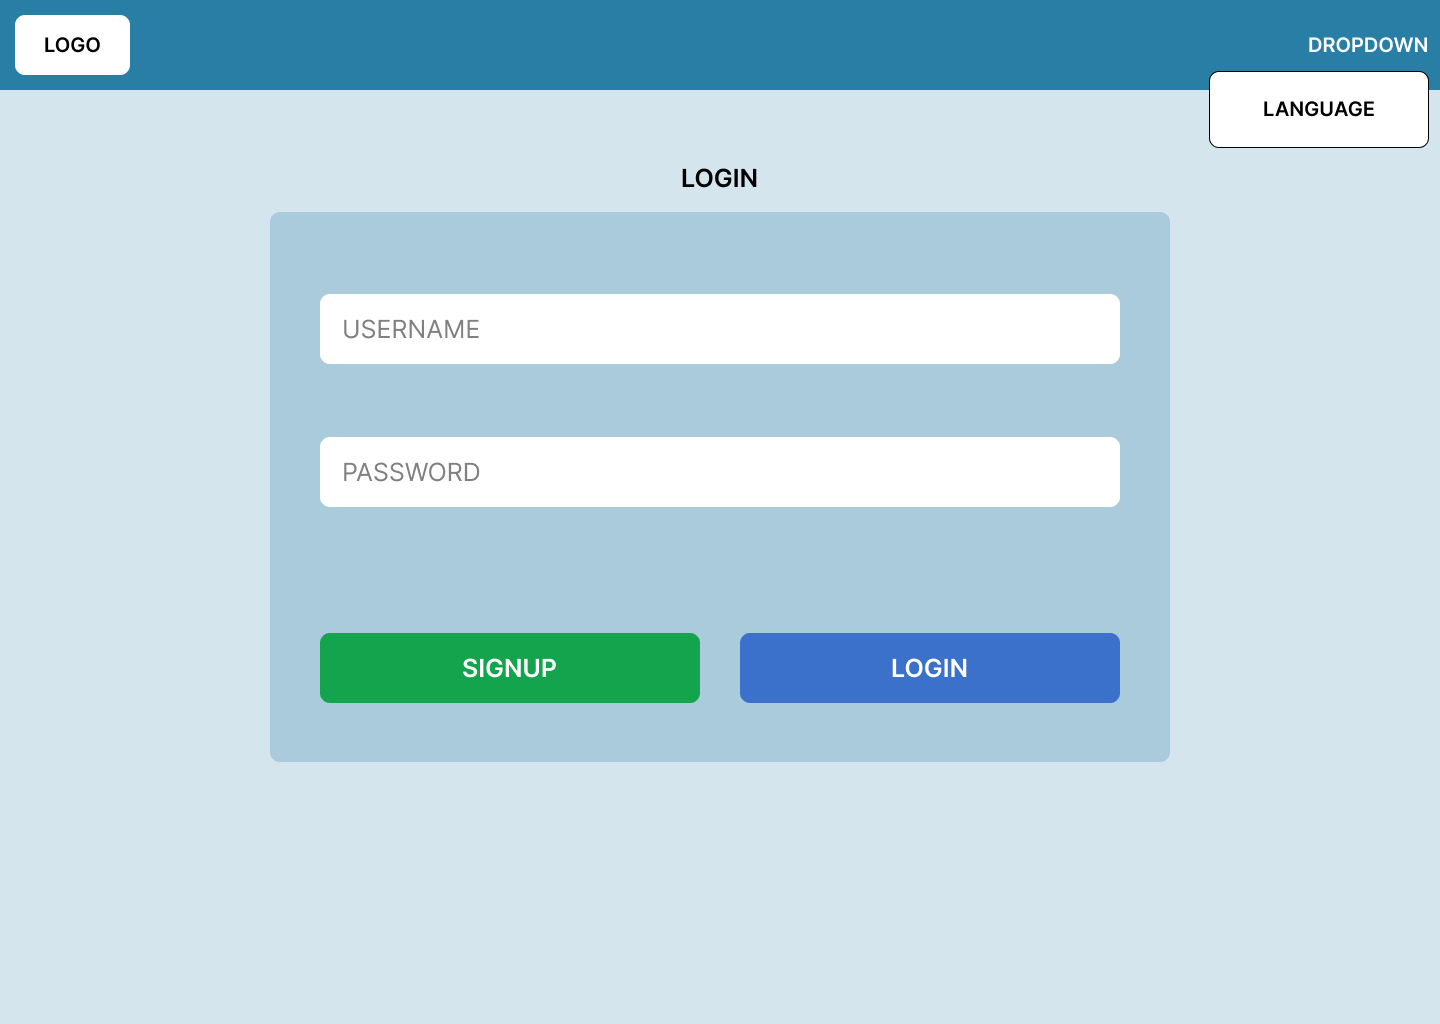
\includegraphics[width=\textwidth]{img/figma/Wireframe-1.png}
\caption{Schermata di login}
\label{fig:pcLogin}
\end{figure}


A seguire una volta effettuato il login l'utente potrà inserire un codice identificativo di una room da creare o alla quale unirsi, attraverso un form visibile nella figura \ref{fig:pcRoom}. Nella stessa figura è mostrata come esempio anche una notifica che il sistema potrà mandare all'utente sfruttando la libreria \emph{react-notifications}\cite{npmjsReactnotifications}.

\begin{figure}[H]
\centering
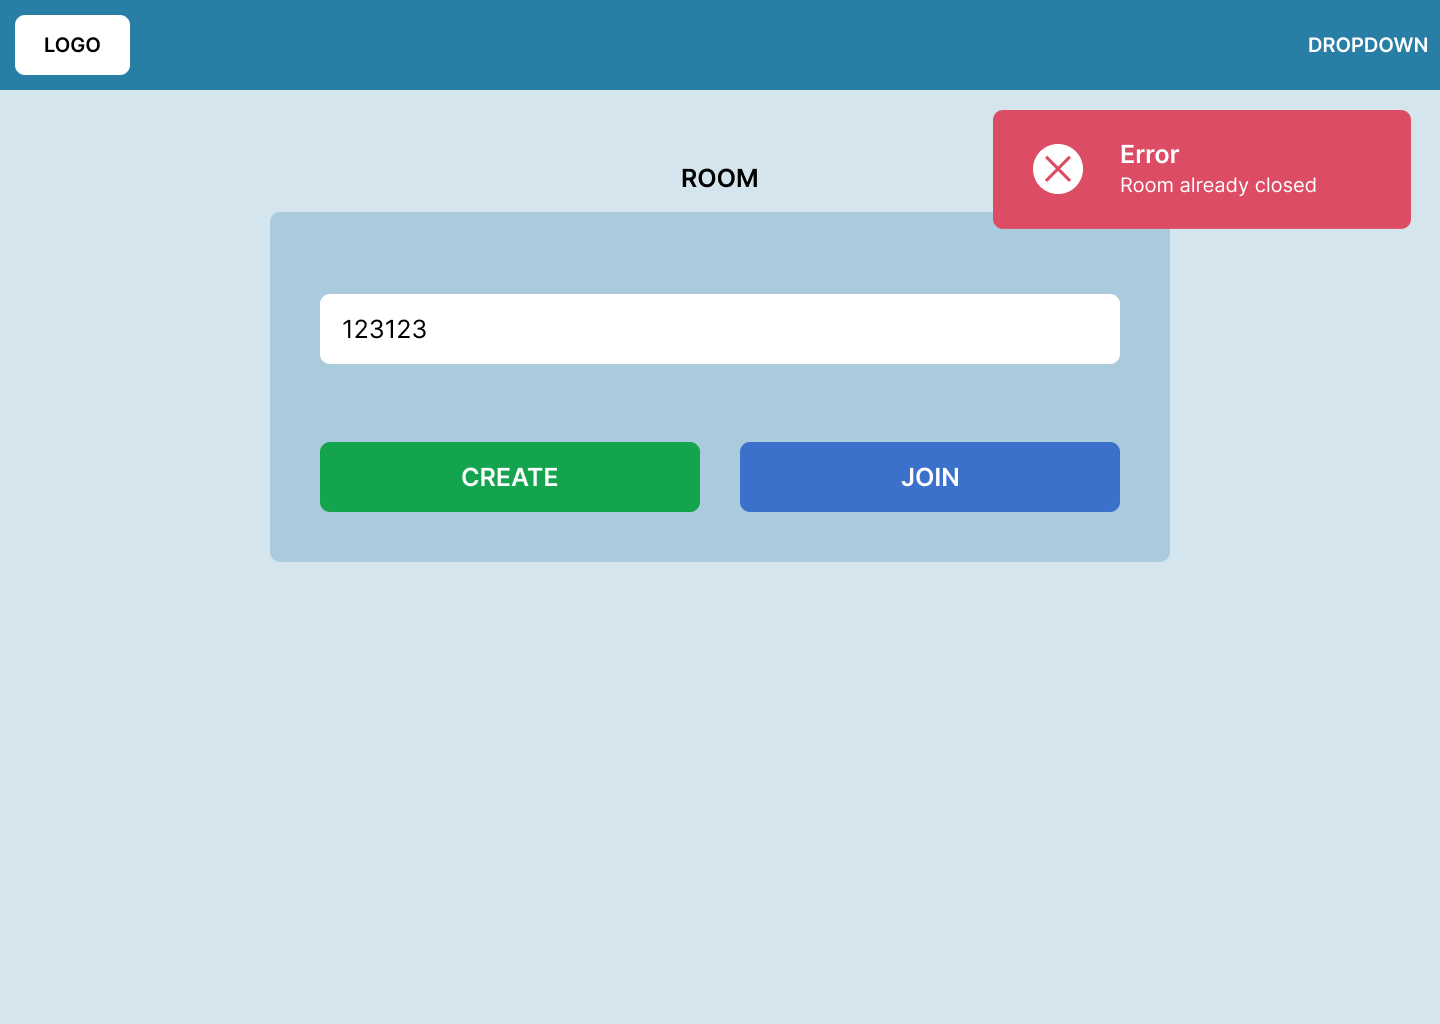
\includegraphics[width=\textwidth]{img/figma/Wireframe-2.png}
\caption{Schermata di selezione della room}
\label{fig:pcRoom}
\end{figure}

\newpage

Una volta all'interno all'utente verrà mostrata una schermata come quella in figura \ref{fig:pcLobby} nella quale si avrà la possibilità di chiudere la room una volta raggiunto il numero minimo di giocatori richiesto. Successivamente in base alle specifiche di implementazione del gioco sarà data la possibilità attraverso un modale di modificare le impostazioni di gioco, come il numero di lupi od eventuali personaggi extra che si vogliono utilizzare.

\begin{figure}[H]
\centering
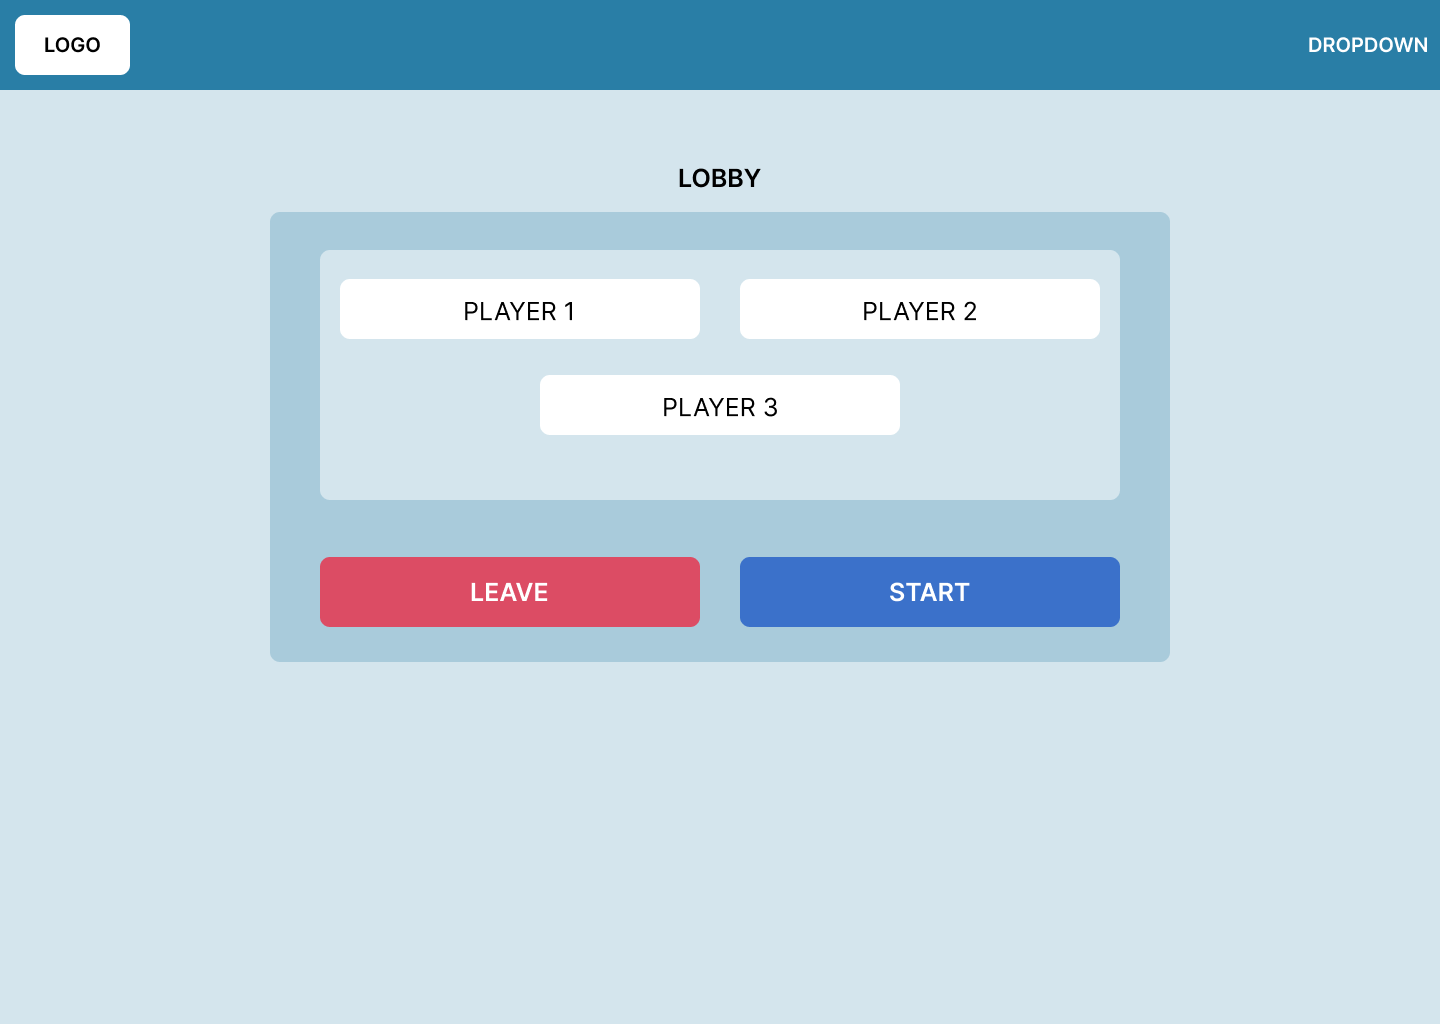
\includegraphics[width=0.9\textwidth]{img/figma/Wireframe-3.png}
\caption{Schermata interna alla room}
\label{fig:pcLobby}
\end{figure}

\newpage

Dopo aver avviato la partita la schermata di gioco sarà quella mostrata nella figura \ref{fig:pcGame}, strutturata su tre colonne contenenti le informazioni necessarie, l'elenco dei giocatori partecipanti, la carta rappresentante il ruolo del giocatore e lo storico degli avvenimenti della partita. In base alla fase di gioco nella parte alta della schermata verrà poi mostrato un ulteriore elenco dei giocatori tra i quali scegliere chi si vuole votare. Nella visualizzazione mobile mostrata nella figura \ref{fig:androidGame} le colonne verranno disposte verticalmente in maniera reattiva in base alla dimensione della finestra.

\begin{figure}[H]
\centering
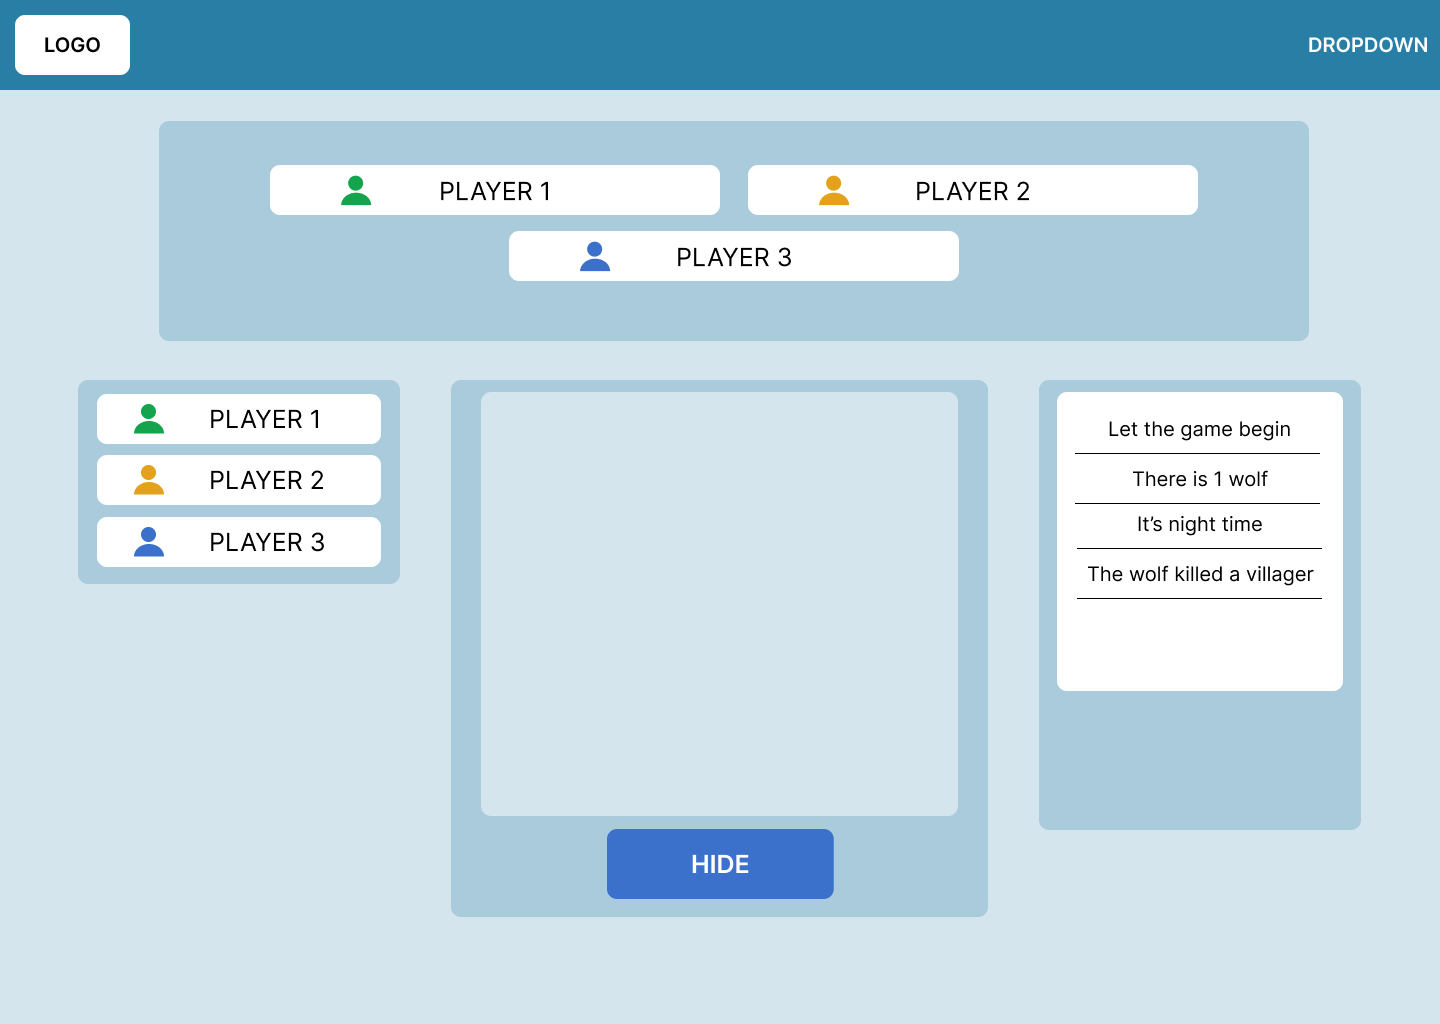
\includegraphics[width=0.9\textwidth]{img/figma/Wireframe-4.png}
\caption{Schermata di gioco}
\label{fig:pcGame}
\end{figure}


\begin{figure}[H]
    \centering
    \begin{minipage}{0.45\textwidth}
        \centering
        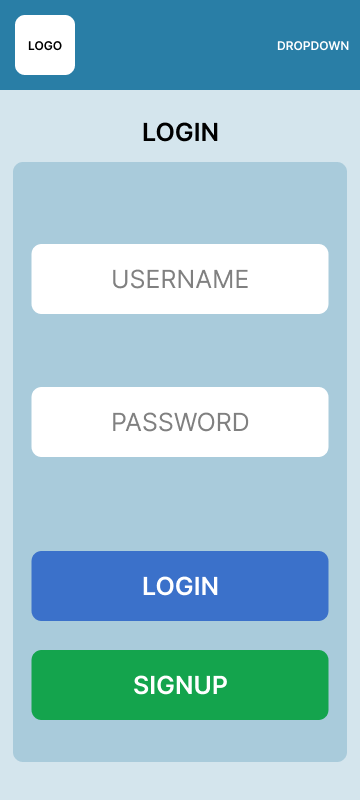
\includegraphics[width=0.9\textwidth]{img/figma/AndroidLarge-1.png} \caption{Schermata di login per dispositivo mobile}
        \label{fig:androidLogin}
    \end{minipage}\hfill
    \begin{minipage}{0.45\textwidth}
        \centering
        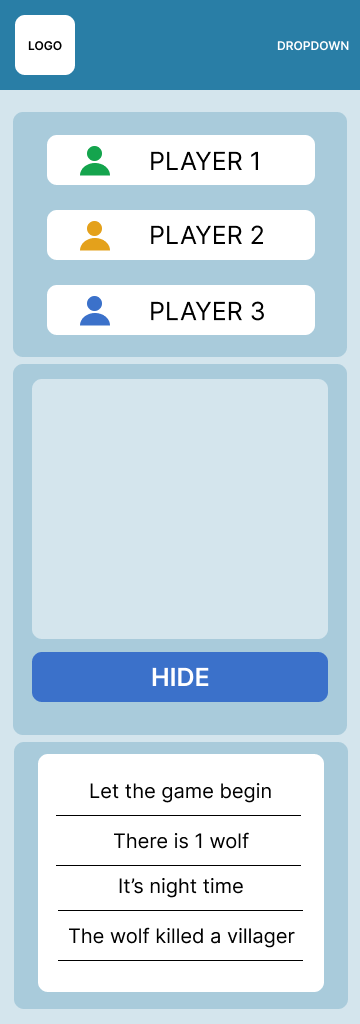
\includegraphics[width=0.9\textwidth]{img/figma/AndroidLarge-2.png} \caption{Schermata di gioco per dispositivo mobile}
        \label{fig:androidGame}
    \end{minipage}
\end{figure}

\newpage

\subsection{Accessibilità}
Durante lo svolgimento di questo progetto i criteri di accessibilità sono stati tenuti in considerazione per ottenere un prodotto finale che li rispettasse al meglio. 
Oltre ai requisiti utili per l'utilizzo di screen reader, come i tag degli elementi ed i testi alternativi alle immagini, è stata posta una particolare attenzione ai contrasti e all'utilizzo dei colori.\\
Alcune di queste scelte sono state prese basandomi sulla mia diretta esperienza in quanto daltonico. La forma di daltonismo più comunemente riscontrata è la deuteranopia (o deuteranomalia), la quale inficia la capacità di distinguere i colori sull'asse rosso-verde. Per questo motivo la palette scelta per le interfacce è stata scelta a partire dal colore identificato da \emph{\#297ea6}, contenente una bassa percentuale di tinta rossa.\\
Per rendere poi accessibile l'applicazione anche a possibili utenti non italiani, come ad esempio studenti in erasmus, in accordo con il concetto di \emph{internationalization} \cite{internationalizationWikipedia} è stata utilizzata la libreria \emph{i18next} \cite{i18next} di react per inserire anche la lingua inglese come alternativa. La schermata di selezione nella sua versione mobile è riportata nella figura \ref{fig:language_mobile}.

\subsection{Interfacce finali}
Le interfacce finali sono riportate al termine della relazione attraverso screenshots della versione desktop e mobile, rispettivamente contenuti nelle appendici \ref{appendix:desktop} e \ref{appendix:mobile}, raccolti durante una demo di gioco.\\

